\section{Experiment Results}
In this section, we will introduce the evaluation results of doctor chatbot and patient chatbot. 

% \KZ{Every human or auto evaluation metric must target one of the
% objectives in Sec 2. Every objective in Sec 2 must be covered by at least
% a human or an auto evaluation. You can have a small table at the beginning
% of this section to align the eval metrics with the objectives. For example,
% the statistics (avg turns etc.) are actually for efficiency, but efficiency
% is not mentioned in the objectives. I think you can include them in sec 2 also.
% Right now the objectives in sec 2 seems to be all language style related.}

\subsection{Doctor Chatbot Results}
% 随着轮数的symptom precision变化
\paragraph{Human Evaluation}
We present the human evaluation results of different doctor chatbots in \tabref{tab:human_doc}. It is evident that ChatGPT-based doctor chatbots outperform the domain-specific data-trained \texttt{CPT} model across various metrics, especially ``fluency'' and ``empathy''. This highlights ChatGPT's ability to control the dialogue flow and provide emotional support. 

However, when comparing the performance of the three ChatGPT-based chatbots (i.e., \texttt{D1}, \texttt{D2}, \texttt{D3}), we find that
\texttt{D3}, which excludes symptom-related aspects from its prompts, outperform the rest in most metrics. Moreover, the chatbot without empathy components, \texttt{D2}, gets the highest score in the ``engagement'' metric. 
% In contrast, the D4 model, trained solely on domain-specific data, may fall short in these areas due to limited diversity and coverage in its training data. As a result, it fails to fully capture the qualities exhibited by human doctors during conversations.
% Chatbots utilizing prompts with empathy components (i.e., \texttt{D1} and \texttt{D3}) are scored higher in ``Empathy'' metrics than other chatbots. 
% Surprisingly, \texttt{D3}, which excludes symptom-related aspects from its prompts, outperform the rest in most metrics. Moreover, the chatbot without empathy components, \texttt{D2}, gets the highest score in the ``Engagement'' metric. 

\begin{table}[th]
    \small
    \centering
    % \resizebox{\columnwidth}{!}{
    \begin{tabular}{l|ccc|c}
    \hline
     & D1 & D2 & D3 & CPT \\ 
     % & (full) & (w/o emp) & (w/o asp) & (cpt)\\
    \hline
    Fluency &3.00	&3.17	&\textbf{3.28}	&2.87 \\
    Empathy &3.36	&3.00	&\textbf{3.43}	&2.71 \\
    Expertise & 2.93	&3	&\textbf{3.71}	&3.29\\
    Engagement & 2.50	&\textbf{3.21}	&2.86	&2.64 \\
    \hline
    \end{tabular}
    % }
    \caption{Human evaluation scores of doctor chatbots}
    \label{tab:human_doc}
\end{table}

As we initially assume that \texttt{D1} with full prompt would deliver the best performance, we reviewed the dialogue history to understand the underlying reason. We found that \texttt{D1} often repetitively expresses empathy, relying on phrases like ``I understand your feelings'' multiple times within a single conversation\footnote{We provide repetitive dialogue examples of doctor chatbots in Appendix \ref{apd:error_anal}.}. This excessive repetition creates the impression that the chatbot lacks a genuine understanding of the patient's issues and relies on pre-written templates, which can negatively impact the user experience.

\paragraph{Automatic Evaluation}
% Then, we continue to explore the dialogue history and calculate some automatic metrics, hoping to find out more reasons of the unexpected human evaluation results. 
The data statistics and automatic metric results are presented in \tabref{tab:auto_doc}, demonstrating a strong correlation with the human evaluation results. 
For example, with automatic metrics, we can explain why \texttt{D3} performs the best in most human metrics. It stands out by asking more in-depth questions while maintaining a lower question frequency per turn, indicating a higher level of professional skills. Furthermore, the symptom precision metric is the highest, implying that the chatbot's questions are highly efficient, with few ``no'' responses.  

These findings validate that the objectives for doctor chatbots proposed with the guidance of psychiatrists, as outlined in \secref{sec:doc_requirements}, effectively capture the requirements of real patients. Therefore, the automatic metrics designed based on these objectives serve as reliable indicators for assessing the performance of chatbots.

\begin{table}[th]
    \small
    \centering
    \resizebox{\columnwidth}{!}{
    \begin{tabular}{l|ccc|c}
    \hline
     & D1 & D2 & D3 & CPT \\ 
     % & (full) & (w/o emp) & (w/o asp) & (cpt)\\ 
    \hline
    - \textbf{Statistics} & & & & \\
        ~~~~avg turns & 25.64&	24.00&	22.71 &	40.93  \\
        ~~~~avg doc utt len &56.84	&57.13	& 53.75	& 14.36\\
        ~~~~avg pat utt len & 8.68	& 10.34	&8.16	&4.87 \\
    \hline
    - \textbf{Function} & & & &   \\
        ~~~~diagnose acc & 42.85\%	& 35.71\%	&\textbf{50.00}\% & 21.43\% \\
    \hline
    - \textbf{Style} & & & & \\
    ~~~~avg \# of ques & 1.6	&1.9	&\textbf{1.22}	&0.92 \\
    ~~~~in-depth ratio & 25.08\%	&27.64\%	&\textbf{32.64}\%	&41.39\% \\
    ~~~~symp recall & 58.93\%	&\textbf{66.07}\%	&38.10\%	&61.90\%\\
    ~~~~symp precision & 72.40\% & 71.93\% & \textbf{92.24}\% & 49.61\% \\
    \hline
    \end{tabular}
    }
    \caption{Automatic evaluation scores of doctor chatbots}
    \label{tab:auto_doc}
\end{table}

Furthermore, we observe that developing a good doctor chatbot is an multi-objective optimization problem, as none of the chatbots can achieve the highest score in all metrics simultaneously.
While high symptom recall and in-depth ratio contribute to a more detailed inquiry, they may inadvertently create a mechanical impression and negatively impact symptom precision. Therefore, achieving a successful doctor chatbot entails striking a careful balance between these objectives.

% However, we also notice some mismatches between the objectives of psychiatrists and the requirements of patients. 
% A notable example is \texttt{D3}, which falls short of psychiatrists' objective of ``comprehensiveness'' due to its low symptom recall caused by the absence of an explicit ``aspect'' component in the prompt. Nonetheless, it can create a more empathetic and understanding experience for patients through its flexible questions that are not constrained by predetermined aspects. In the face of such mismatches, we should prioritize experts' opinions to ensure that the diagnosis process adheres to medical standards, rather than solely catering to user preferences. 

\begin{figure*}[th]
	\centering
	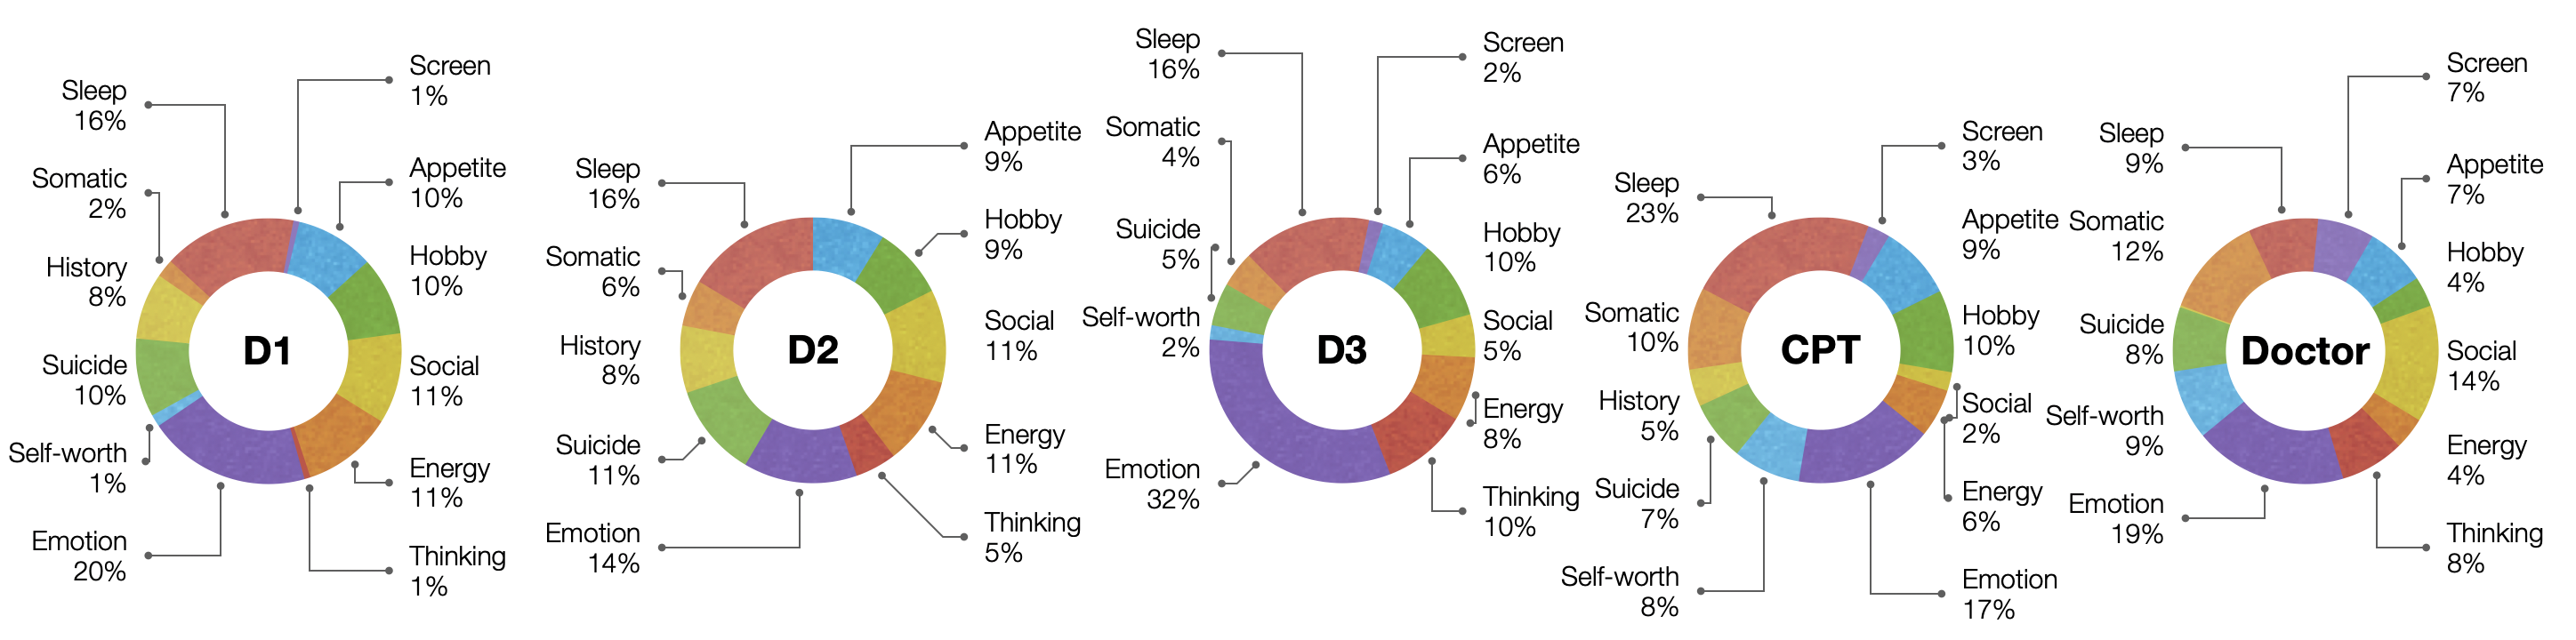
\includegraphics[width=\linewidth]{Figures/topics.png}
	\caption{The proportion of symptoms asked by different doctor chatbots and human doctor.}
	\label{fig:symp_anno}
\end{figure*}


% We can find that \texttt{D3} has the fewest average number of dialogue turns and the least amount of text per turn among all the ChatGPT-based bots. Additionally, it tends to ask more in-depth questions while asking fewer questions each turn, both of which indicate higher professional skills as a psychiatrist. 
% \KZ{Asking in-depth questions seems to contradict with shorter text per turn.
% That's why you better show some examples to clear these doubts.}
% Furthermore, the symptom precision metric is the highest, suggesting that the chatbot's questions are highly efficient, with few ``no'' responses.  
% \KZ{Is there a particular order in which the doc bot follows in asking questions? I guess, when doc asks questions, they go from very general questions, down 
% to specific ones, like navigating down a tree structure. They should ask 
% questions adaptively according to the patients response. I wonder if our
% design permits this kind of style.}
% However, as the required aspects are not explicitly stated in the prompt, the symptom recall metric of this chatbot is relatively low, indicating that its diagnosis may not be comprehensive enough. Nevertheless, the chatbot's questions are more flexible and free-flowing, precisely because there are no predetermined aspects to ask. As a result, patients feel more understood, leading to a better experience overall.

% What's more, \texttt{D2} received the longest responses from patients, which is consistent with the human evaluation metric ``Engagement'', suggesting that patients are more willing to converse with this chatbot. 
% It also achieves the highest symptom recall among all the chatbots, even surpassing \texttt{D1} which also includes aspects in the prompt. 
% This could because \texttt{D1} contains too many instructions regarding empathy and other factors, which may have hindered its ability to thoroughly inquire about all the required symptoms.


\begin{figure*}[th]
 	\centering
	\begin{subfigure}{0.36\linewidth}
		\centering
		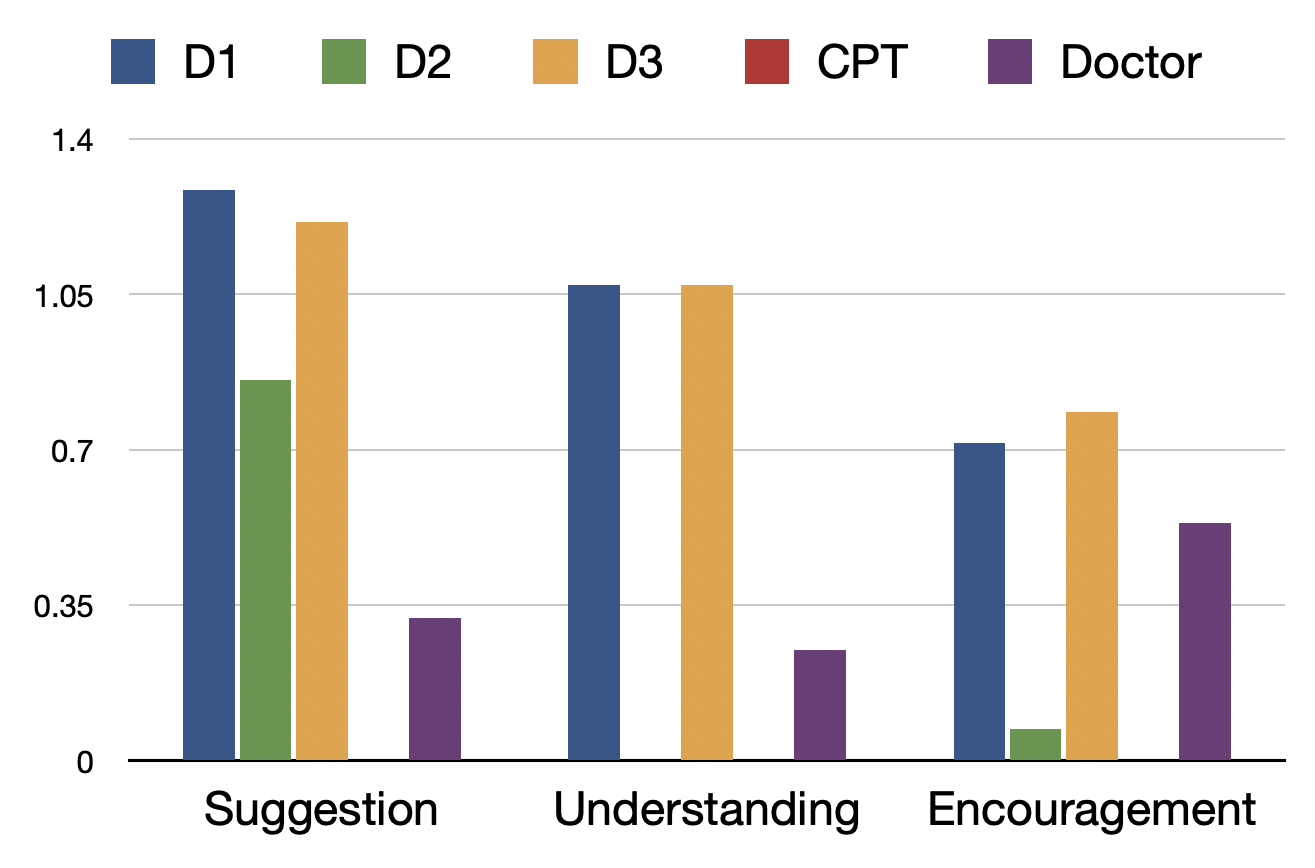
\includegraphics[width=\linewidth]{Figures/empathy.png}
		\caption{Empathy Behaviors}
		\label{fig:emp_simu_doctor}%文中引用该图片代号
	\end{subfigure}
	\centering
	\begin{subfigure}{0.36\linewidth}
		\centering
		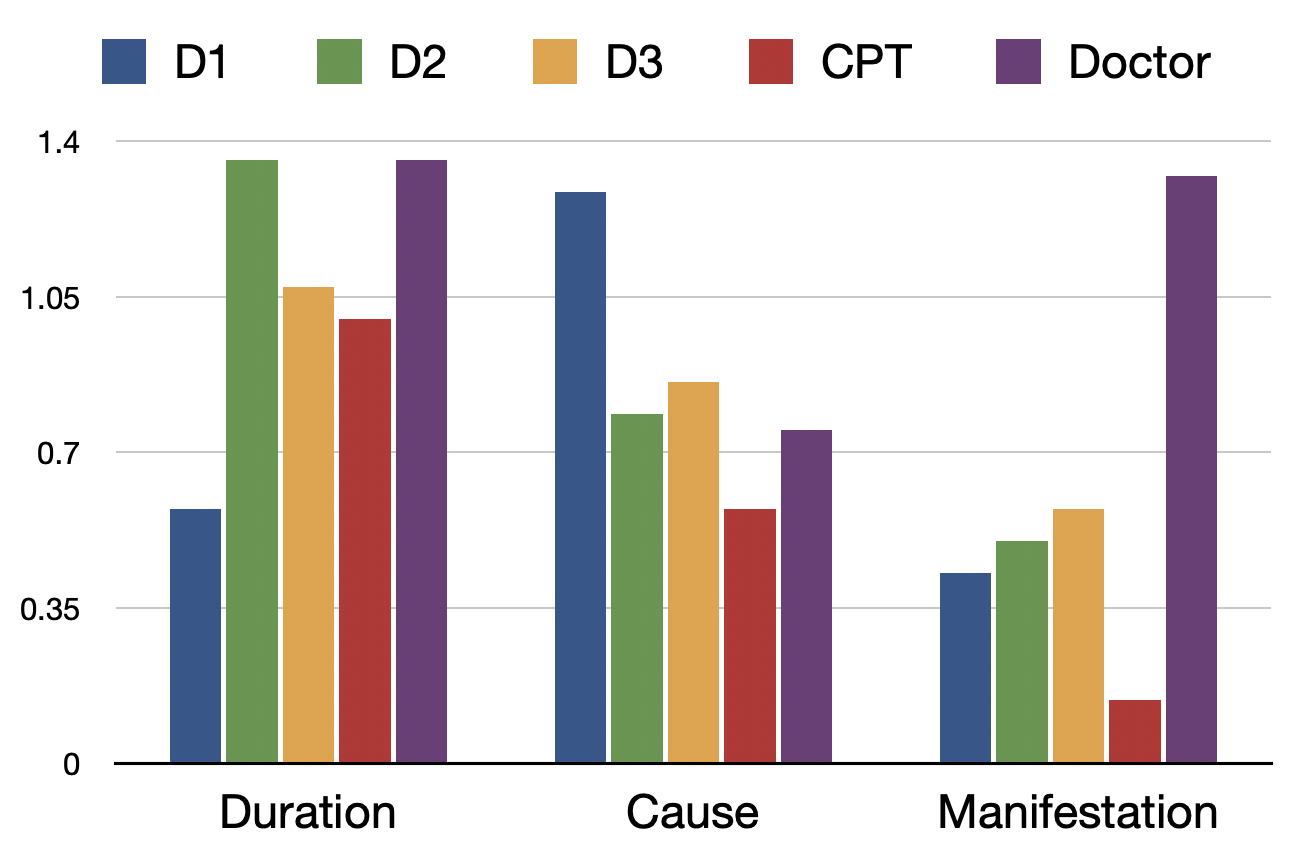
\includegraphics[width=\linewidth]{Figures/indepth.png}
		\caption{In-depth Question} 
		\label{fig:indepth_simu_doctor}%文中引用该图片代号
	\end{subfigure}
	\caption{Dialogue act comparison between different doctor chatbots and human doctor. The y-axis means the average number of the behavior occurs in the dialogue history.
 % \KZ{What is the y axis of these figs?}
 }
	\label{fig:doctor_chatbot_statistics}
\end{figure*}
% NEWCOMMENT: 图片的纵轴是什么?

\subsection{Human vs. Doctor Chatbots}
\label{sec:comp_doctor}

By involving human doctors in conversations with patient chatbots, we can identify the limitations of doctor chatbots by comparing them to the ideal benchmark represented by human doctors. We analyze their behaviors based on three dimensions: topic proportion, empathy behaviors and in-depth questions, using the annotated dialogue history\footnote{We discuss the details of the annotation in Appendix \ref{apd:annotation}.}.
% COMMENT: 这里和patient chatbots的关系是?“标注question topic和dialogue act”也出现得有些突兀。应该先说要从这两方面对比评估,再说要标注其类型,可能会更顺畅一些?
% COMMENT: 有doctor chatbot与patient chatbot对话的实验吗?如果没有的话,这里的实验设计得会不会有什么问题?
% NEWCOMMENT: 这里的对比还是很奇怪,评价doctor chatbot是通过和人类病人聊天的,而人类医生是和机器人病人聊天的,该变量未控制的话,这个对比合理吗?
% NEWCOMMENT: 一个很自然的质疑就是,既然patient chatbot和真实病人是有差异的,那么在该变量未控制的情况下,有没有可能是谈话对象的不同导致了采取的对话策略不同呢?怎么证明这个对比反映的一定是doctor chatbot和人类医生的内在能力的差异呢?

\paragraph{Topic Proportion}
% Accordingly, we calculated the average proportion of question topics of different doctor chatbots, as well as human doctors. \figref{fig:symp_anno} displays the outcomes. 
In \figref{fig:symp_anno}, most doctor chatbots tend to inquire more thoroughly about emotion and sleep-related symptoms. Human doctors, on the other hand, have a more even distribution of questions about various symptoms.
Moreover, human doctors often do ``screening'' to rule out other possible conditions (see the examples in Appendix \ref{apd:human_doc_example}), while chatbots rarely exhibit such behavior, indicating the possible limitations in multi-disease scenarios~\cite{Zhang2022SymptomIF}.

\paragraph{Empathy Behaviors}
% Then we calculated the average number of empathetic strategies utilized by doctors in the dialogue history, as illustrated in Figure . 
\figref{fig:emp_simu_doctor} shows that \texttt{D1} and \texttt{D3} can utilize a range of empathetic strategies, while \texttt{D2} only offers suggestions to patients because the empathy instructions in prompt are removed. Moreover, though human doctors use all the strategies, their usage is less frequent than that of chatbots. This is because chatbots often strive to understand and empathize without considering appropriateness, whereas human doctors will choose suitable moments for empathetic interactions.

% When asked for the reasons behind this, doctors attributed it to the limited inquiry time in real outpatient scenarios and the bias resulting from the difference in interaction with chatbots compared to real people~\cite{Yun2021BehavioralAN}.

\paragraph{In-depth Questions}
% Further, we also calculated the various ways of in-depth questioning, and obtained Figure \ref{fig:indepth_simu_doctor}.
% \KZ{How did you count the number of in-depth questions? Automatically or manually? By looking for keywords?Is it accurate?} 
\figref{fig:indepth_simu_doctor} reveals that the frequency of asking about the duration or cause of symptoms is similar between human doctors and chatbots. However, human doctors ask significantly more questions about the specific manifestations of each symptom than chatbots do, as this helps to better understand the vague expressions of patients.

\subsection{Patient Chatbot Results}

\paragraph{Human Evaluation}
The human evaluation results of patient chatbot are in Table \ref{tab:human_pat}. It can be observed that all metrics of \texttt{P2}
% \MY{Following my previous comment in listing these in a table, I would suggest you using very brief abbreviations and include them in this table, e.g. D1, D2 and P1, P2 and just use these abbr. for all the later texts.} 
are higher than \texttt{P1}. This suggests that the inclusion of resistance, colloquialism, etc., makes the chatbot more similar to real patients, according to the doctors' perspective.
% COMMENT: and so on -> etc.?

\begin{table}[ht]
    \small
    \centering
    % \resizebox{\columnwidth}{!}{
    \begin{tabular}{l|cc}
    \hline
     & P1 & P2 \\ 
    \hline
    Resemblance & 1.93 & \textbf{2.21} \\
    ~~~~Mental State & 2.07 & \textbf{2.42} \\
    ~~~~Life Experience & 2.00 & \textbf{2.14}  \\
    ~~~~Expression style & 1.57 & \textbf{2.21} \\
    \hline
    Rationality & 2.42 & \textbf{2.57}  \\
    \hline
    \end{tabular}
    % }
    \caption{Human evaluation scores of patient chatbot.}
    \label{tab:human_pat}
\end{table}

\paragraph{Automatic Evaluation}
We show the results of automatic metrics in Table \ref{tab:auto_pat}. It appears that ``unmentioned symptom ratio'' of \texttt{P2} is higher than \texttt{P1}, indicating a higher level of resistance. We also find that \texttt{P2} engages in slightly more dialogue turns with longer responses from the doctor than \texttt{P1}. This may be attributed to the inclusion of resistance in the prompt, which requires the psychiatrists to provide more guidance and encourage the patient chatbot to share more information. 
% The statistics of empathy strategies used by the psychiatrists in the conversation with these two patient chatbots can further support this point, which will be discussed in Section \ref{sec:comparison}.

%In informal conversations, people often rely on a smaller set of daily words and phrases. %This limited range of vocabulary contributes to less diversity in spoken language compared to written language.
% Since spoken language typically has less diversity than written language, \KZ{is there any ref for this? I don't see why spoken language is less diverse than
% written.}
What's more, \texttt{P2} has more human-like words and fewer robot-like words, echoing the higher human evaluation score in the dimension of ``expression style'', which indicates that its language style is more colloquial compared to \texttt{P1}. To effectively showcase the resistance behaviors and emotional expressions of the patient chatbot, we include several examples in Appendix \ref{apd:examples}.

However, we observe that \texttt{P2} performs less competitively in the ``wrong symptom ratio'' metric, indicating that it may report more symptoms that are not included in the patient portrait. One possible reason for this could be the excessive focus on language style and resistance in the prompt, which might cause ChatGPT to ``forget'' the actual symptoms of the patient. 

% We  in Appendix \ref{apd:examples}, which can provide a more intuitive and comprehensive understanding of different chatbots.
% xd\MY{there are too many newly-named metrics, we NEED to align the automatic and subjective metrics to objectives in Sec2. You can either categorise doctor and patient ones into function and style, or they can name as the objectives. After aligning these, our contribution can have corresponding adjectives for the doctor and patient bots.}


\begin{table}[th]
    \footnotesize
    \centering
    % \resizebox{1.05\linewidth}{22mm}{
    \begin{tabular}{l|cc}
    \hline
    & P1 & P2 \\ 
    \hline
    - \textbf{Statistics} & & \\
    ~~~~avg turns & 31.64 & 33.36\\
    ~~~~avg patient utt len & 40.38 & 40.94 \\
    ~~~~avg doctor utt len & 16.74 & 17.38 \\
    \hline
    - \textbf{Function} & & \\
    ~~~~wrong symp ratio & \textbf{15.07\%} & 18.38\%   \\
    \hline
    - \textbf{Style} & & \\
    % ~~~~Distinct-1 & 42.6\% & \textbf{37.3\%}  \\
    ~~~~human-like word num & 5.36 & \textbf{10.29}   \\
    ~~~~robot-like word num & 7.21 & \textbf{3.79} 	  \\
    ~~~~unmentioned symp ratio &  9.12\% & \textbf{12.28\%} \\
    \hline
    \end{tabular}
    % }
    \caption{Automatic evaluation scores of patient chatbot}
    \label{tab:auto_pat}
\end{table}

% \subsection{Human vs. Patient Chatbot}
% \label{sec:comparison}

% Similarly, as we invited real patients to participate in the evaluation, we can compare the language style of real patient and patient chatbots. 
